\section{AutoLibra\protect
\includegraphics[height=1em]{figs/scale.png}}

\begin{figure}[!t]
    \centering
    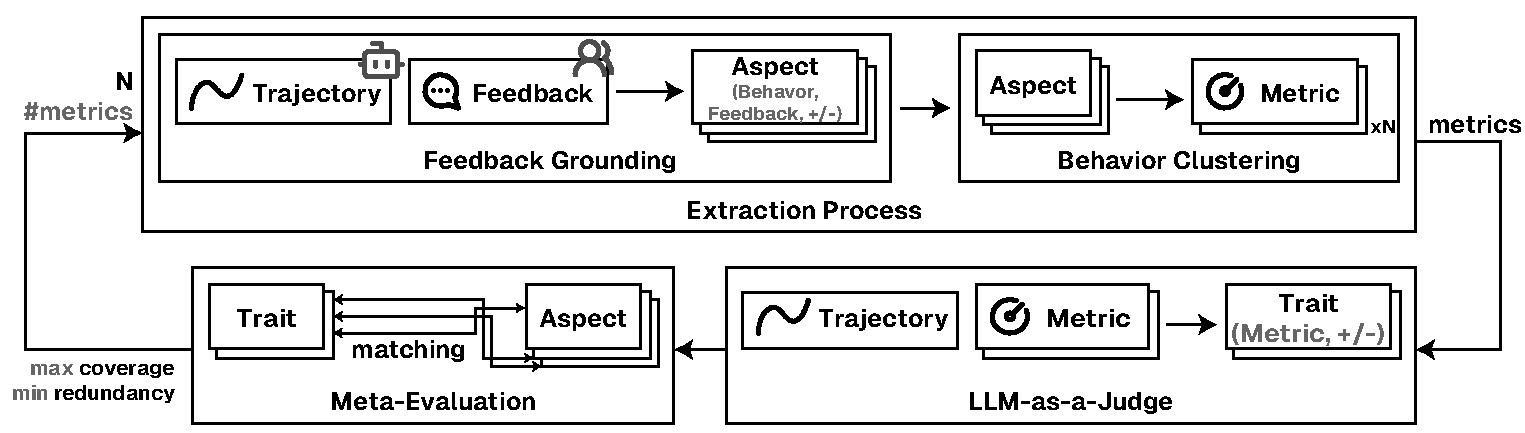
\includegraphics[width=\textwidth]{figs/autolibra-pipeline.pdf}
    \caption{AutoLibra pipeline. AutoLibra consists of three major components: Extraction Process
    turns annotated agent trajectories into metrics, LLM-as-a-Judge evaluates the agent trajectories
    based on the induced metrics, and Meta-Evaluation Process measures the quality of induced metrics
    through matching the detect agent traits with grounded feedback aspects.
    }
    \label{fig:autolibra-pipeline}
\end{figure}

To address the limitations of existing evaluation paradigms, we seek to design an evaluation method that 
meets the following desiderata: (1) \emph{data-driven}: this makes sure that the metrics are grounded
in the real agent behavior and human opinions, (2) \emph{generic}: applicable to various agent domains 
without the need for domain-specific design, (3) \emph{self-verifiable}: this provides guarantee that the 
induced metrics can be used in LLM-as-a-Judge to generate human-aligned evaluation. 

As illustrated in Fig. \ref{fig:autolibra-pipeline}, AutoLibra achieves these desiderata through a closed-loop pipeline
consisting of three major steps: \textbf{Extraction Process} first grounds the human feedback
for each trajectory into aspects (\S\ref{sec:grounding}), and then clusters the aspects into $N$ metrics (\S\ref{sec:clustering}).
\textbf{LLM-as-a-Judge} gives each trajectory scores for the induced metrics, the combinations of
metrics and scores becoming the traits of the agents (\S\ref{sec:llm-judge}).
Finally, \textbf{Meta-Evaluation Process} measures the quality of induced metrics through matching
the detected agent traits with aspects in the human feedback (\S\ref{sec:meta-evaluation}).
To optimize for the lowest redundancy with highest coverage, we control the number of metrics 
through a hyperparameter $N$ in the clustering step (\S\ref{sec:metric-optimization}). AutoLibra also supports
an interactive metric induction process, where as the agent is optimized, new metrics can be added
to the existing metrics (\S\ref{sec:iterative-induction}).

\subsection{Feedback grounding}
\label{sec:grounding}
The feedback of human annotators could contains multiple aspects, e.g. \textsf{``AI agent was pretty good
on giving me a consistent itinerary and vacation plan, although It froze on the last couple of minutes.''},
collected from human annotators in CoGym \citep{shao2024collaborative}, contains a positive aspect
about the agent's ability to generate a consistent itinerary, and a negative aspect about the agent freezing
at the end. Here we define an \emph{aspect} as a triple $(\texttt{behavior}, \texttt{feedback}, \texttt{sign})$.
In the positive aspect of the previous example, the \texttt{behavior} is the agent's actions to create
a 20-day itinerary for Maldives, the \texttt{feedback} is that the itinerary created is consistent, 
and the \texttt{sign} is positive. This grounding procedure is similar to coding in thematic analysis.

In this step, we not only feed the trajectory and feedback into the LLM (we use GPT-4o \citep{openai2024gpt4ocard} 
as it yields good results in our experiments), but also provide the LLM with the following instructions:
(1) break down the feedback into bulletpoints; (2) for each bulletpoint, find the corresponding
part of the trajectory that the feedback is referring to. Finally, we use constrained decoding to force GPT-4o
to output the aspects in the previous format. In our experiments, we find that on most datasets, for each
trajectory, the LLM can generate one to five aspects, with an average number of one to two aspects per trajectory.


\subsection{Behavior clustering}
\label{sec:clustering}

The second step of the Extraction Process is to cluster the aspects into $N$ metrics.
To illustrate this step, we consider another example in the same dataset
\textsf{The AI responds quickly to write and run the Python script.} where
the \texttt{behavior} is the agent's action to quickly write and run a Python script, the \texttt{feedback}
is that the agent responds quickly, and the \texttt{sign} is positive. Although this aspect is a positive aspect,
it reflects the same dimension of the agent's behavior as the previous negative aspect just on the opposite side.
Each \emph{metric} is a cluster of aspects, with a definition summarizing the criteria of positive behaviors,
and a list of positive behavior examples, and a list of negative behavior examples. This clustering procedure
is similar to the theme induction step in thematic analysis.

However, clustering similar agent behaviors together is challenging for statitiscal clustering methods.\footnote{
    In preliminary experiments, we tried to use K-means clustering on the aspect vectors generated by \texttt{text-embedding-3-large},
    but the clusters are mostly based on tasks and not on the behaviors.
}
Inspired by \citet{viswanathan2024large,lam2024concept}, we prompt an LLM
(we use o3-mini high\footnote{https://openai.com/index/openai-o3-mini/}, as it yields the best coverage and redundancy scores
    as evaluated later) to cluster the aspects 
into $N$ metrics, and provide the LLM with the following instructions:
The granularity of the grouping should be minimal, only very similar behaviors should be grouped together.
But don't limit to one particular website or one particular character.


\subsection{LLM-as-a-Judge}
\label{sec:llm-judge}

LLM-as-a-Judge \citep{zheng2023judging},
or more broadly model-based evaluation 
\citep{zhang2019bertscore,celikyilmaz2021evaluationtextgenerationsurvey}
is a method to use machine learning models to evaluate the output of other machine learning models.
The success of it depends on the gap between the difficulty of the evaluation or verification and 
that of generation and action. 
In agentic tasks, this gap is often large, as the policy model needs to perform 
multiple steps of decision making, while the evaluation model only needs to
classify the trajectories, which make LLM-as-a-Judge widely used \citep{zhouwebarena,he2024webvoyager,zhousotopia}.
In AutoLibra, we also use LLM-as-a-Judge to
evaluate the agent trajectories configurated with the induced metrics. However, LLM-as-a-Judge
can be replaced by any other evaluation methods implementing the induced metrics,
e.g. \texttt{interact-valid-element} metric
could be evaluated by a rule-based evaluator which checks if the agent
interacts with valid elements on the webpage. Future research could explore
programmtical evaluation generation methods \citep{maeureka} to generate 
programs for the induced metrics.

Taking the induced metrics as input, an LLM (we use o3-mini medium,
as it provides similar results in this step as o3-mini high
but is cheaper to run) is prompted to rate agent trajectories into
\{+1, -1, N/A\} for each metric. The output of LLM-as-a-Judge is a set of
positive \emph{traits}, and a set of negative \emph{traits}. When we calculate the scores of 
the metrics, we use the ratio of agent trajectories rated as positive
to the ones that are rated as positive or negative, ignoring the N/A ones,
since not all metrics are applicable to all trajectories ---
some metrics like \texttt{valid-search-terms} are only applicable when the task
involves searching. 

\subsection{Meta-evaluation}
\label{sec:meta-evaluation}

The last component of the loop is the Meta-Evaluation Process. ``Meta'' here implies 
that we are evaluating the evaluation metrics and results. 
This step takes the traits detected by the LLM-as-a-Judge, and matches them with the aspects
grounded from the human feedback. The goal is to verify (1) whether the induced metrics 
covers what the human annotators care about, and (2) whether LLM-as-a-Judge can produce
accurate evaluation results based on the induced metrics. In the previous example,
if the \texttt{respond-promptly} is extracted as a metric, and the LLM-as-a-Judge
has the same opinion as the human annotators, then this aspect is considered as successfully covered.
If either a similar metric was not extracted, or the LLM-as-a-Judge assigns a different score,
then this aspect is considered as not covered.

To perform this step, we separate the aspects into positive and negative aspects, and
traits into positive and negative traits, and only try to match the positive aspects with positive traits,
and negative aspects with negative traits. 
We prompt an LLM (we use GPT-4o \citep{openai2024gpt4ocard},
as it yields good results in our experiments) with a list of aspects and another list of traits,
and ask the LLM to find the best matching trait for each aspect or decide that there is no matching trait.
The \emph{coverage} of the whole dataset is calculated as the proportion of aspects that have a matching trait,
and the \emph{redundancy} is calculated as the proportion of traits that have not been matched to any aspect.


\subsection{Metric optimization}
\label{sec:metric-optimization}
We aim at prioritizing coverage of the metrics to provide comprehensive evaluation of the agent behavior,
while minimizing the overlap within the metrics to avoid redundancy.
To optimize for this objective, we generate 20 different metrics with $N$ ranging from 4 to 13,
and calculate the coverage and redundancy of the metrics on the human feedback.
We then select the metrics with a coverage of at least the highest coverage minus 1\%,
and the lowest redundancy.
This is performed iteratively, by resetting the range of $N$ to the number of metrics selected
previously plus or minus 2, and repeating the process until the coverage and redundancy
of the selected metrics do not change significantly, normally within 3 iterations.
This optimization process is a very simple strategy. We have also tried various other optimization
strategies, including genetic algorithms --- sythesizing new metrics by combining the existing ones,
and iterative clustering --- iteratively cluster unmatched aspects into new metrics, but none of them
yield better results than the simple strategy.

\subsection{Iterative metric induction while agent improves}
\label{sec:iterative-induction}
When applying AutoLibra to agent optimization, we can iteratively induce new metrics as agents could
have new failure modes or new behaviors as they improve.
For example, in the Baba-is-AI task \citep[\S\ref{sec:baba-is-ai}]{cloos2024babaaibreakrules},
agent initially fails to recognize the win condition and act randomly,
after agent improves with an in-context example in the prompt, the agent starts to 
follow existing win conditions, but fails to construct new win conditions.
This was not mentioned in human feedback before the agent improvement, since the agent
was too random to even reach the stage where constructing new win conditions is possible.
Therefore, a new metric \texttt{win-rule-construction} should be induced in the second iteration 
to provide a new signal for optimizing the agent even further.

Although instead of adding new metrics, we can also induce a complete new set of metrics from scratch
in each iteration, adding new metrics to the existing ones is useful for tracking agents' progress
across different iterations. In practice, we do not find this results in any coverage loss. 
To do this, we slightly change the behavior clustering step, by providing the LLM with the existing metrics
and their definitions, and ask the LLM to not change the definitions of the existing metrics, 
only add new examples to the existing metrics and add new metrics if necessary.
We apply the same optimization strategy as in the metric optimization step
to make sure the newly induced metrics do cover emerging behaviors and not overlap with the existing metrics.

\begin{table}[!t]
    \centering
    \small
    \begin{tabular}{ccccccc}
        \toprule
        Steps & CoGym & Sotopia & WebArena & WebVoyager & Baba-is-AI & MiniHack  \\
        \midrule
        Grounding & 0.95 & 0.95 & 0.98 & 0.93 &  &  \\
        LLM-as-a-Judge & 0.90 & 0.85 & 0.95 & 1.00 &  & \\
        Meta-Evaluation & 0.98 & 0.90 & 0.85 & 0.83 &  &  \\
        \bottomrule
    \end{tabular}
    \caption{
        The ratio of instances marked as fully correct in human validation. For each step and
        each task, we randomly sample 40 instances and ask human annotators to label them as completely correct
        or not. Although the agreement scores vary across tasks and steps, the average agreement for each
        step and dataset is above 0.9. 
}
    \label{tab:validation}
\end{table}

\subsection{Collecting human feedback and validating AutoLibra}
\label{sec:collecting-human-feedback}

In this paper, we use two kinds of human feedback for different kinds of agent. (1) Agents that directly interact
with humans: we use the feedback from the users who are interacting with the agents. CoGym \citep{shao2024collaborative}
is the setting belongs to this category, and we use the user comments collected in their study. (2) Agents that 
do not directly interact with humans: we use the feedback from human annotators who observe the agent trajectories.
The annotators are instructed to explicitly point out the aspects of the agent behaviors that they think are good or bad,
and refrain from giving a very general comment like \textsf{The agent is good at solving the task}
but instead give a more specific comment like \textsf{The agent cannot figure out how to get to the other room}.
The annotators can also choose from a TTY and a web interface, on both of which they first check out the agent's task,
and then view the agent's observation and actions step by step. Although for web navigation tasks, viewing screenshots
is more straightforward, we keep the observation format the same as the one we used for the agents. 
For multi-agent tasks, we annotate each agent's trajectories separately.

To answer the question of whether AutoLibra is aligned with human judgment,
we validate the feedback grounding, LLM-as-a-Judge, and meta-evaluation steps through another human annotation process.
We did not validate the behavior clustering step, as it is super hard for human annotators to
process more than 400 aspects and perform clustering on them. The coverage and redundancy scores
together with validation results of the other steps in the loop can serve as an indirect validation for the 
behavior clustering step.
Table \ref{tab:validation} shows the agreement rate of the human annotators on the AutoLibra steps. 
It should be noted that these tasks are vastly different, e.g. grounding for WebVoyager \citep{he2024webvoyager} is quite hard 
due to the complexity of the trajectory, and LLM-as-a-Judge for Sotopia \citep{zhousotopia} is 
difficult due to the complexity of the evaluating social interaction. 